\section{Observation}
	Least Count of Calibrated Drum = $(\delta \lambda)$ = $1\;nm$\\\\
	\textbf{Table for calibration using mercury lamp:}

	\begin{table}[H]
		\centering
		\begin{tabular}{|c|c|c|}
		\hline
		\textbf{Sl. No} & $\lambda_{given}$ (nm) & $\lambda_{given}$ (nm) \\ \hline
		1 & 546 & 546 \\ \hline
		2 & 577 & 577 \\ \hline
		3 & 579 & 579 \\ \hline
		4 & 502 & 493 \\ \hline
		5 & 435 & 437 \\ \hline
		\end{tabular}%
		\caption{Calibration using Hg lamp}
		\label{tab:calib}
	\end{table}

	\begin{figure}[H]
		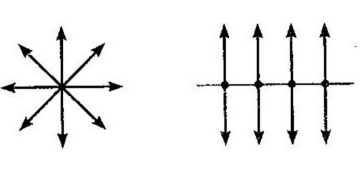
\includegraphics[width=\columnwidth]{calibration.png}
		\caption{$\lambda_{given}(l)\;vs\;\lambda_{observed} (L)$ Plot}
		\label{graph:calib}
	\end{figure}

	\vspace{-1cm}
	\noindent $\lambda_{corrected} = m\lambda_{observed} + c$\\
	From the Graph we Get:\\
	\indent slope $(m) = 1.003 \pm 0.041$\\
	\indent intercept $(c) = -3.079 \pm 21.925$


	\textbf{Table for emission spectrum of metals:}
	\begin{itemize}
		\vspace{-5mm}
		\item \textbf{For Copper:}
		\vspace{-5mm}
		\begin{table}[H]
			\centering
			\begin{tabular}{|c|c|c|c|}
			\hline
			\textbf{Sl.No} & \textbf{$\lambda_{observed}$   (nm)} & \textbf{$\lambda_{corr}$   (nm)} & \textbf{$\lambda_{lit}$   (nm)} \\ \hline
			1 & 511 & 509 & 510 \\ \hline
			2 & 516 & 514 & 515 \\ \hline
			3 & 523 & 521 & 522 \\ \hline
			4 & 570 & 569 & 570 \\ \hline
			5 & 578 & 577 & 578 \\ \hline
			\end{tabular}
			\caption{Emission Spectrum for Copper}
			\label{tab:copper}
		\end{table}
		
		\vspace{-1.5cm}
		\item \textbf{For Brass:}
		\vspace{-5mm}
		\begin{table}[H]
			\centering
			\begin{tabular}{|c|c|c|c|}
			\hline
			\textbf{Sl.No} & \textbf{$\lambda_{observed}$   (nm)} & \textbf{$\lambda_{corr}$   (nm)} & \textbf{$\lambda_{lit}$   (nm)} \\ \hline
			1 & 510 & 508 & 510 \\ \hline
			2 & 516 & 514 & 515 \\ \hline
			3 & 523 & 521 & 522 \\ \hline
			4 & 570 & 569 & 570 \\ \hline
			5 & 577 & 576 & 578 \\ \hline
			6 & 637 & 636 & 636 \\ \hline
			8 & 474 & 472 & 472 \\ \hline
			\end{tabular}
			\caption{Emission Spectrum for Brass}
			\label{tab:brass}
			\end{table}
	\end{itemize}

	\vspace{-1cm}
	\textbf{Table for absorption spectrum of iodine:}
	\vspace{-5mm}
	\begin{table}[H]
		\centering
		\begin{tabular}{|c|c|c|c|c|}
		\hline
		Sl.No & \begin{tabular}[c]{@{}c@{}}$\lambda_{observed}$\\ (nm)\end{tabular} & \begin{tabular}[c]{@{}c@{}}$\lambda_{corr}$\\ (nm)\end{tabular} & \begin{tabular}[c]{@{}c@{}}Wave number\\ $\bar{\nu_e}\;(cm^{-1})$\end{tabular} & \begin{tabular}[c]{@{}c@{}}Wave number\\ $\delta\bar{\nu_e}\;(cm^{-1})$\end{tabular} \\ \hline
		1  & 563 & 562 & 17806 & --    \\ \hline
		2  & 566 & 565 & 17711 & 95  \\ \hline
		3  & 568 & 567 & 17648 & 63  \\ \hline
		4  & 572 & 571 & 17524 & 124 \\ \hline
		5  & 575 & 574 & 17432 & 92  \\ \hline
		6  & 578 & 577 & 17341 & 91  \\ \hline
		7  & 582 & 581 & 17222 & 120 \\ \hline
		8  & 585 & 584 & 17133 & 89  \\ \hline
		9  & 589 & 588 & 17016 & 117 \\ \hline
		10 & 593 & 592 & 16900 & 115 \\ \hline
		% 11 & 597 & 596 & 16787 & 114 \\ \hline
		% 12 & 600 & 599 & 16702 & 84  \\ \hline
		% 13 & 604 & 603 & 16591 & 111 \\ \hline
		% 14 & 609 & 608 & 16454 & 137 \\ \hline
		% 15 & 613 & 612 & 16346 & 108 \\ \hline
		% 16 & 617 & 616 & 16240 & 107 \\ \hline
		% 17 & 621 & 620 & 16135 & 105 \\ \hline
		% 18 & 625 & 624 & 16031 & 104 \\ \hline
		\end{tabular}
		% \caption{Absorption Spectrum for Iodine}
		\label{tab:iodine}
		\end{table}
	

	\begin{table}[H]
		\centering
		\begin{tabular}{|c|c|c|c|c|}
		\hline
		Sl.No & \begin{tabular}[c]{@{}c@{}}$\lambda_{observed}$\\ (nm)\end{tabular} & \begin{tabular}[c]{@{}c@{}}$\lambda_{corr}$\\ (nm)\end{tabular} & \begin{tabular}[c]{@{}c@{}}Wave number\\ $\bar{\nu_e}\;(cm^{-1})$\end{tabular} & \begin{tabular}[c]{@{}c@{}}Wave number\\ $\delta\bar{\nu_e}\;(cm^{-1})$\end{tabular} \\ \hline
		% 1  & 563 & 562 & 17806 &     \\ \hline
		% 2  & 566 & 565 & 17711 & 95  \\ \hline
		% 3  & 568 & 567 & 17648 & 63  \\ \hline
		% 4  & 572 & 571 & 17524 & 124 \\ \hline
		% 5  & 575 & 574 & 17432 & 92  \\ \hline
		% 6  & 578 & 577 & 17341 & 91  \\ \hline
		% 7  & 582 & 581 & 17222 & 120 \\ \hline
		% 8  & 585 & 584 & 17133 & 89  \\ \hline
		% 9  & 589 & 588 & 17016 & 117 \\ \hline
		% 10 & 593 & 592 & 16900 & 115 \\ \hline
		11 & 597 & 596 & 16787 & 114 \\ \hline
		12 & 600 & 599 & 16702 & 84  \\ \hline
		13 & 604 & 603 & 16591 & 111 \\ \hline
		14 & 609 & 608 & 16454 & 137 \\ \hline
		15 & 613 & 612 & 16346 & 108 \\ \hline
		16 & 617 & 616 & 16240 & 107 \\ \hline
		17 & 621 & 620 & 16135 & 105 \\ \hline
		18 & 625 & 624 & 16031 & 104 \\ \hline
		\end{tabular}
		\caption{Absorption Spectrum for Iodine}
		% \label{tab:iodine2}
		\end{table}